\section{Visualization Design}
\begin{figure*}[t]
	\centering
    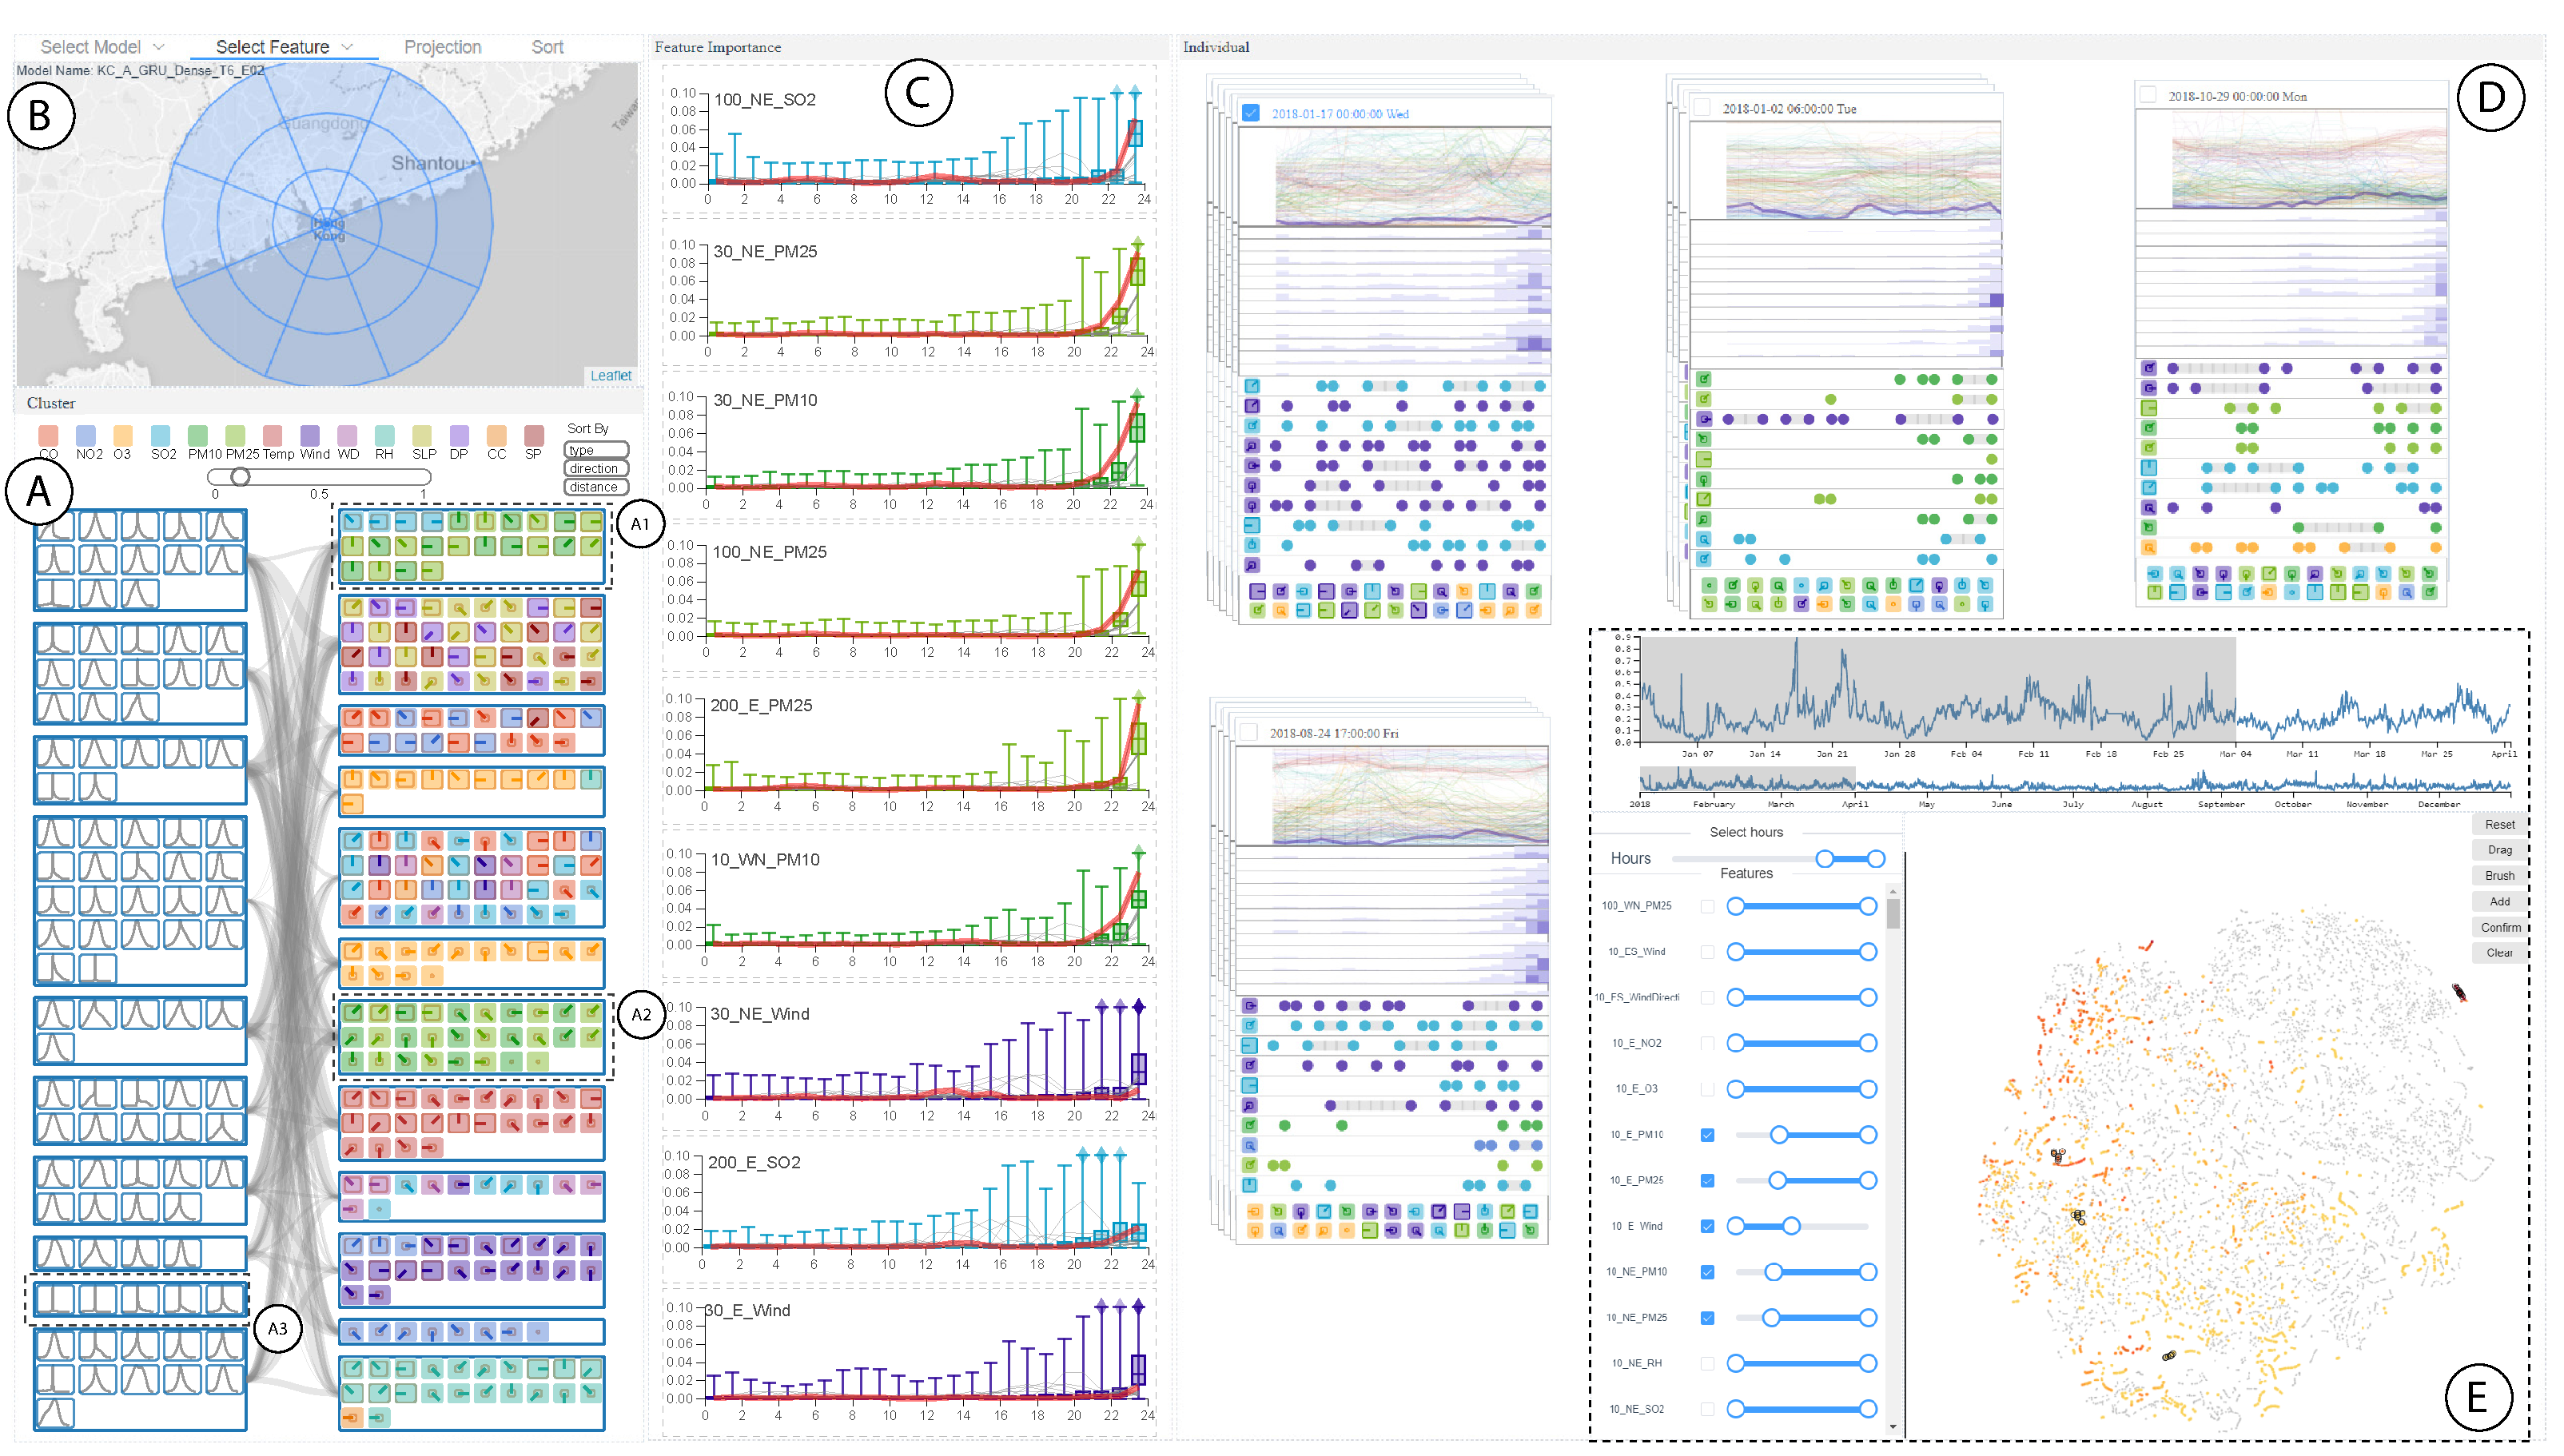
\includegraphics[width=0.95\textwidth]{pictures/teaser.pdf}
	\vspace{-3mm}
	\caption{MultiRNNExplorer contains multiple coordinated views to support exploring and understanding RNNs' behaviors on multi-dimensional time-series data, especially on hidden unit response and feature importance. The Configuration Panel (B) allows users to select an RNN model and configure parameters.  To reveal model mechanism, the Cluster View (A) summarizes the hidden unit clusters' response to feature clusters, and the Feature Importance View (C) summarizes the temporal importance of input features.  The Projection View (E) displays a data overview, allowing users to select sequence instances of interest for further analysis.  The selected instances will be shown in the Individual View (D).}
	\label{fig:teaser}
	\vspace{-4mm}
\end{figure*}


In this section, we introduce the visual design based on the design tasks discussed in Sec.\ref{section:design_tasks}.  As shown in Fig.~\ref{fig:teaser}, the visual analytic system consists of six coordinated views. Starting from the configuration panel Fig.~\ref{fig:teaser}B, users are able to select the target feature and the model to be analyzed. The region partition will be shown as Fig.~\ref{fig:teaser}B after the model is selected. To support exploring the model mechanism, the Cluster View is displayed to summarize the hidden units' response to the features (Fig.~\ref{fig:teaser}A) and the Feature Importance View (Fig.~\ref{fig:teaser}C) is shown to visualize the temporal importance of each feature. Furthermore, users can select the individual cases in the Projection View (Fig.~\ref{fig:teaser}E) and the selected cases are grouped by similarity and displayed in the Individual View (Fig.~\ref{fig:teaser}D).

%!TEX root = ../article.tex
\subsection{Cluster View}
% To enable users to observe the statistics of both the features and hidden states (\textbf{T1},\textbf{T2}), we develop the Cluster View (Fig.~\ref{fig:teaser}).
% It shows the overview of response relationship (\textbf{T3}) between the hidden units and features. The hidden units and features are visualized as the Hidden State Distribution and the Feature Glyph respectively.

The Cluster View (Fig.~\ref{fig:teaser}A) shows the overview of response relationship (\textbf{T3}) between the hidden units and features. The hidden units and features are visualized as the Hidden State Distribution and the Feature Glyph respectively.


\begin{figure}[t]
	\centering
    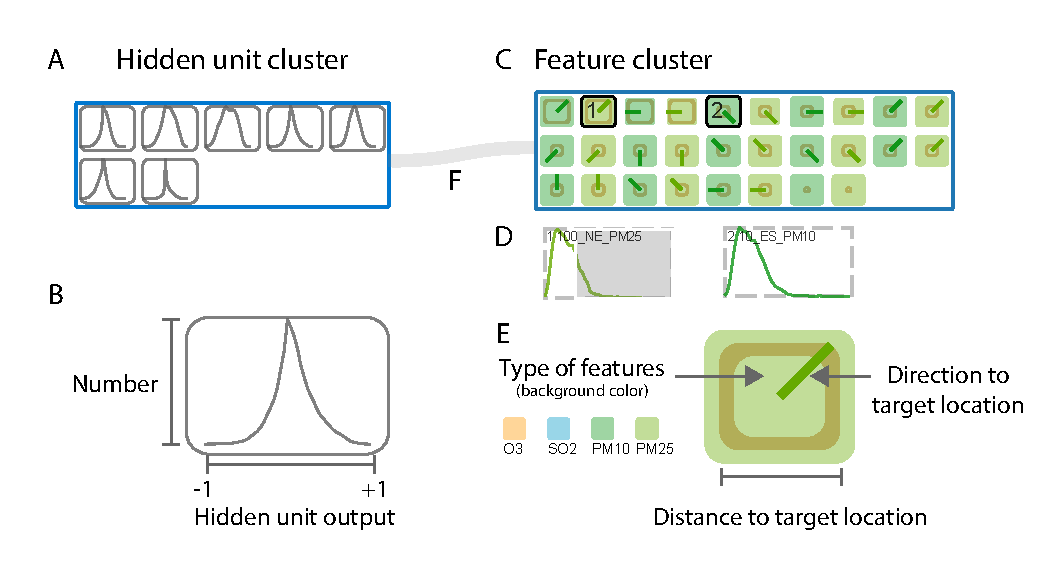
\includegraphics[width=0.45\textwidth]{pictures/design/cluster_design.pdf}
	\vspace{-3mm}
	\caption{Design of Hidden unit distribution and feature glyph. A) Hidden unit cluster; B) Hidden unit distribution; C) Feature cluster; D) Feature distribution for selected features; E) Feature glyph design; G) Response link}
	\label{fig:cluster_design}
	\vspace{-4mm}
\end{figure}


\textbf{Hidden State Distribution.}
The left column on the Cluster View is the Hidden State Distribution component.
As shown in Fig.~\ref{fig:cluster_design}A, each row represents a hidden unit cluster.
% The row height increases with the number of hidden states in each cluster.
Each hidden unit in a cluster is represented as a line chart that shows its activation distribution(\textbf{T1}).
The x-axis represents the hidden unit output ranging from $-1$ to $+1$ and the y-axis represents the \UC{corresponding probability} (Fig.~\ref{fig:cluster_design}B).
From the line chart, users can observe and compare the activation distribution patterns of different hidden units. 

\textbf{Feature Glyph.}
The right column of the Cluster View is the Feature Glyph component (Fig.~\ref{fig:cluster_design}C).
Similar to the Hidden State Distribution, each row represents a feature cluster in which a glyph (Fig.~\ref{fig:cluster_design}D) represents a feature.
\yh{This enables users to quickly identify different features and compare the common attributes of multiple features for analysis.}
\yh{As described in Sec.~\ref{section:application}, we define our usage scenario as air pollution forecasting where each feature has three identifiers: the feature category, the direction, and the distance from the feature to the target location.}
\yh{As a categorical feature, we first use the background color of the feature glyph cell to encode the feature category.
Different hues encode different categories, and users can find the color legend at the top of the Cluster View.}
\yh{To intuitively encode target location direction, we draw a line segment starting from the glyph center that has the same direction angle.
We also draw a square in the glyph where its radius, which is an appropriate channel to encode numerical values, encodes the distance to the target location.}

% In each feature glyph, the distance and direction to the target location are presented by a rectangle and a line segment with one end point at the center.
% The angle of the direction bar encodes the direction, and the width of the distance rectangle represents the distance(Fig.~\ref{fig:cluster_design}D).

\textbf{Interactions.}
We also support various interactions to allow users to dynamically explore this view.
The curves linking the hidden state cluster and feature cluster with the width indicate the response strength (Fig.~\ref{fig:cluster_design}E). Users can also filter the link according to the response strength by adjusting the slider bar. 
When hovering over a hidden state cluster or a feature cluster, the corresponding links and linked clusters will be highlighted.

In this view, the users can obtain an overview of the response relationship between hidden units and features, for example, we can find that there are not strong links connecting to cluster 8 (Fig.~\ref{fig:teaser} A$_3$), this may be because that all the hidden units are ``weakly'' activated in cluster 8.
% Users can also select a feature for further examination by clicking the corresponding feature cell.
% After clicking, a line chart will be appended to the right of the Feature Distribution component (Fig.~\ref{fig:cluster_design}D) to show the feature's value distribution.

\subsection{Feature Importance View}
The feature importance view allows users to explore the feature contribution to model output (\textbf{T2}).
As discussed in Sec.\ref{section:feature_importance}, with an input case, we are able to measure the importance of a single feature as a sequence of importance scores which correspond to the importance at all timestamps (Fig.~\ref{fig:teaser}C). 

Since the importance score only provides a local description for the feature importance, an effective visualization is needed to show an overview of each feature's importance. We choose boxplot for this task since it can present the statistics overview. To show the temporal trend of a feature, we group the importance score of all test cases by the timestamps and make statistics group by group. For the test sequence with a length $T$, will use the feature importance charts which contain $T$ boxplots to show the trend of feature importance (Fig.~\ref{fig:teaser}C).

The horizontal axis indicates the timestamps and the vertical axis indicates the feature importance score. The top line, upper edge, middle line, bottom edge and bottom line of the boxplot indicate the maximum,  $75^{th}$ percentile, mean, $25^{th}$ percentile and minimum of the importance scores.  Since sometimes the maximum will much larger than the $75^{th}$  percentile value, which makes the box vary flat and difficult for users to explore the temporal pattern, we limit the maximum score $Ms$ shown in the view. If a boxplot has scores larger than $Ms$, a diamond symbol appears on the top of the boxplot. The opacity of the diamond indicates the magnitude of the absolute difference between the largest score and $Ms$.    

We also define the overall importance score for a single feature as the sum of the mean score at all timestamps. By default, the boxplot charts will be ranked according to the overall feature importance score. Due to the large number of features, only the top 10 feature importance charts are visualized. Users may observe other features by using the scroll bar or filtering the features from the projection view (Fig.~\ref{fig:teaser}C). 


%!TEX root = ../article.tex
\subsection{Projection View}
To help users obtain an overview of case clusters and outliers (\textbf{T5}), we design the Projection View (Fig.~\ref{fig:teaser}E) which supports various interactions such as zooming and brushing to allow users to select a subset of data for further examination.

In the Projection View, each circle represents a individual case. There are many multi-dimensional reduction methods such as MDS and PCA; we select t-SNE as it can strongly repel dissimilar points and show clusters clearly.
For each case, we collect the feature cluster importance over all time steps (discussed in Sec.\ref{section:feature_importance}) as the input vectors of t-SNE.
% \QM{Given an individual case, we flatten the cluster importance at all timestamps (discussed in Sec.\ref{section:feature_importance}) to 1-dimensional as the t-SNE embedding vector.}
% \yh{?}
Thus, the positions of the circles reflect the similarity of their cluster importance.
\QM{We use a sequential color to encode the model's output of each case.}
\yh{$<$to discuss: sequential color scheme description?$>$}
% Add to increase the space
% When multiple data subsets are selected, we use a categorical color scheme to fill the circles so that the data sequences from the same data subset will have the same color in both components.
% Users can brush to select data sequences for detailed examination in the Sequence View.

% One major consideration in developing the Projection View is the scalability problem.
% When the number of circles is large, the circles may overlap with each other, and the Projection View can be cluttered.
% We adopt a node overlap removal algorithm for the similarity projection and support panning and zooming to allow users to explore a data subset.

Furthermore, to improve the flexibility of the case selection, we add a two-scale timeline (Fig.~\ref{fig:teaser}E~top) to show the target feature trend, enabling user filtering of the cases by time, and a feature selection component (Fig.~\ref{fig:teaser}E~left) to filter the cases by feature value.  


%!TEX root = ../article.tex
\subsection{Individual View}
After observing an overview on data similarities, users may need to drill down to a few individuals of interest for detailed examination.
We develop the Individual View for users to explore and compare the different individuals over time (\textbf{T6}).
Specifically, our goal is to identify the important features at different time steps and their relationship to raw feature values (\textbf{T2}, \textbf{T4}).


\begin{figure}[t]
	\centering
    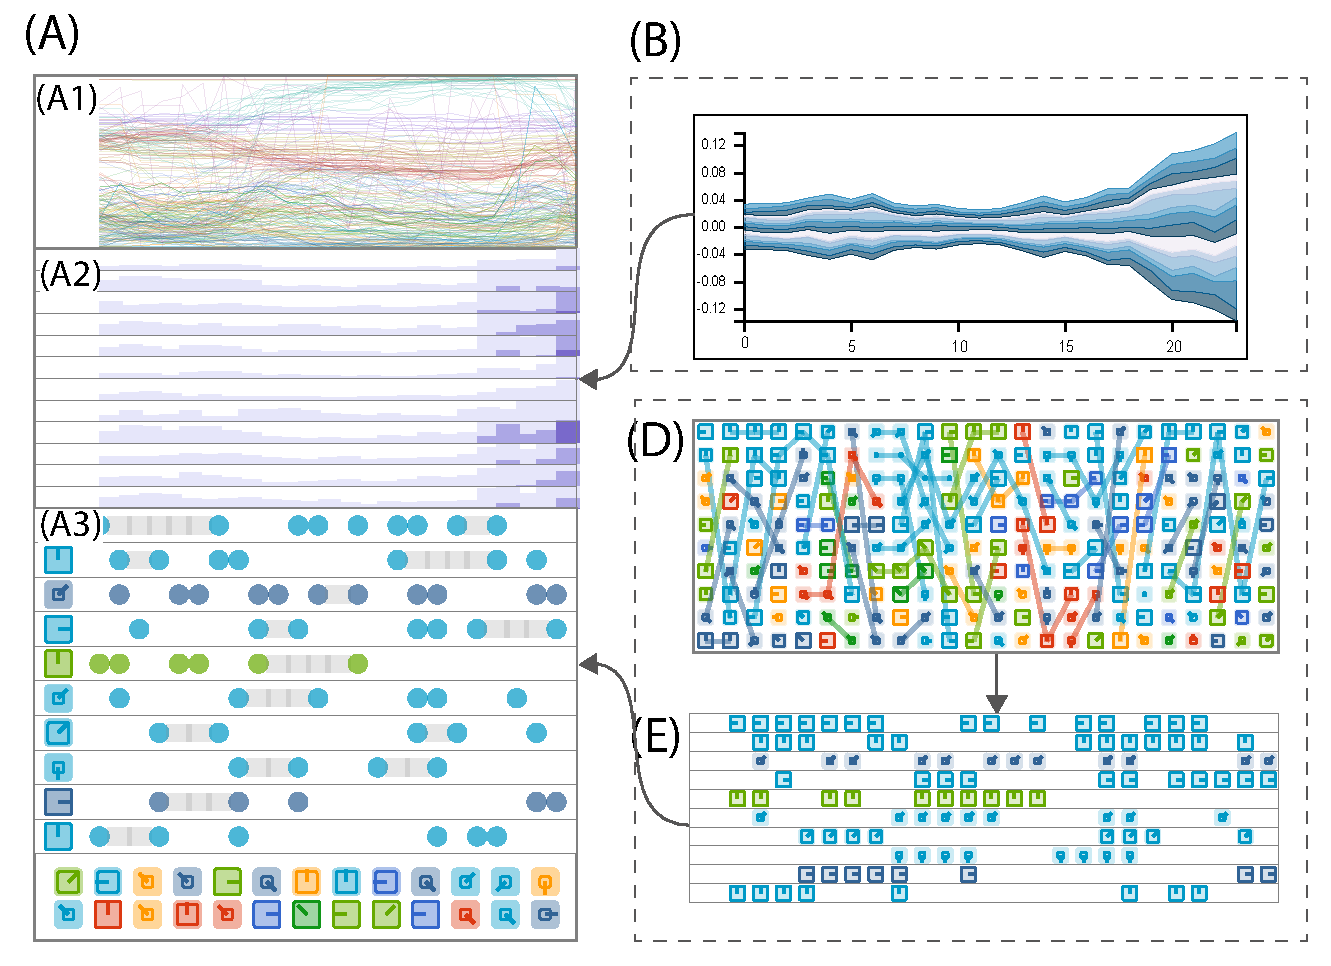
\includegraphics[width=0.49\textwidth]{pictures/design/alternative_design.pdf}
	\vspace{-3mm}
	\caption{Individual design and the alternative designs. A) Individual View. A1) Feature Trend Chart; A2) Cluster Importance Chart; A3) Top Features Chart. B) themeriver as the alternative design of the Cluster Importance Chart; C) and D) node-like sequence and node sequence as the alternative design of Top Features List.}
	\label{fig:individual_view}
	\vspace{-4mm}
\end{figure}


The selected individual cases are visualized as several stacks of cells as in Fig.~\ref{fig:individual_view}A to show the detailed information.
Each cell consists of three components: the Feature Trend Chart, the Cluster Importance Chart, and the Top Feature List from top to bottom as shown in Fig.~\ref{fig:individual_view}A$_1$,A$_2$,A$_3$.
The top component is the Feature Trend Chart, which is a multi-line chart that depicts how different features' values change over time. 
The x-axis represents the time where time steps increase from left to right, and the y-axis represents normalized feature values where the feature value increases from bottom to top ranging between 0 and 1.
Each line represents a feature and the line color encodes feature category the same as in the Cluster View.
The corresponding lines will be highlighted when hovering on any feature groups in the Cluster View to enable users to focus on the features in the current context and avoid visual clutter.

The middle component is the Cluster Importance Chart, which is a list of stacked bar charts that summarize how each feature group's gradient changes over time.
Each feature group is represented as a stacked bar chart and aligned vertically in the same order as the Cluster View.
For each bar chart, the x-axis represents time the same as in the Feature Trend Chart, and each bar represents the averaged gradient for the corresponding feature group at one time step. 
We use both the bar height and bar color to encode the gradient value.
As shown in  Fig.\ref{fig:individual_view}A$_3$, the first visual channel to encode gradient value is bar height where a greater height indicates a larger gradient value.
When the gradient value exceeds a certain limit, we clip the bar and overlay another darker bar with the same height as the clipped part at the same position for better vertical space efficiency.
We have also considered other design choices such as a themeriver (Fig.\ref{fig:individual_view}B) in which each colored flow indicates a feature group. 
However, users may feel it is difficult to compare different feature groups, and it requires more space when the gradient is large.
Thus, we abandon this alternative choice and adopt the current design.

Though the Cluster Importance Chart provides an overview of how each feature cluster's importance changes over time, users still need to link this component to the Cluster View to observe which features are considered important by the model.
We first design a Top Feature List as shown in Fig.~\ref{fig:individual_view}D. We rank the features by importance at each timestamp, and only visualize the top N features by layout feature glyph for each timestamp in order to alleviate the burden on users. If a feature is ranked in the top N important features for more than two consecutive timestamps, we use a link to connect the adjacent glyph. However, this design also leads to serious visual clutter caused by the link overlap, since the rank of features are frequently only slightly changed by timestamps. 
To alleviate the user's mental burden, we improve the Top Feature List as Fig.~\ref{fig:individual_view}A$_3$ shows.
In this component, we visualize the top $N$ features that have the largest average gradients over time. Each feature is represented as a horizontal row and the glyph appears at the timestamps when this feature is ranked in the top $K$($K>N$) most important features (Fig.\ref{fig:individual_view}E). To further simplify the visual design, the feature glyph is positioned at the beginning to indicate feature category. 
As a feature has different gradients over time, the importance ranking of a feature can also vary at different steps.
For each row, we use two colored circles linked with gray lines to indicate at which time steps the corresponding feature is ranked in the top $K$($K>N$) mostly important features.
The circle color is consistent with the feature glyph color.
To make the Top Feature List space efficient, we only show ten feature rows by default, and other features are collapsed as feature glyph rows as shown in the bottom at Fig.\ref{fig:individual_view}A$_3$.
Users can click the glyph rows to select different features to analyze.


The three components enable users to observe which features are considered important by the model over time and how the importance is related to feature value changes.
Users can also append multiple cells to the Sequence View to compare different sequences side by side. 
When the number of cells becomes large, we use dbscan to cluster the similar individual cases into one stacked cells with one randomly selected case presented at the top of stack.
\subsection{Interactions and Linkage}
To better facilitate the interactive exploration of RNNs, our system supports cross-view interactions. In this section, we summarize the interactions and linkage among all four views.

\textbf{Cross-view highlight.} 
In summary, there are three key visualization components appearing across different views: \textbf{feature}, \textbf{feature cluster} and \textbf{case}. These components are visualized in different forms in different views to support various analysis requirements. For example, a feature is visualized as a glyph (Fig.\ref{fig:cluster_design}E) in the cluster view,  visualized as a series of boxplots (Fig.\ref{fig:teaser}C) in the Feature Importance View and shown as both a line chart (Fig.\ref{fig:individual_view}A$_1$) and a sequence (Fig.\ref{fig:individual_view}A$_3$) in the individual view. If one feature is selected by mouse hover, the corresponding visualization element in other views will be highlighted with a border stroke.

\textbf{Linkage between individual view and feature importance view.} 
When multiple individual cases are selected, in addition to visualizing these cases in individual views, the feature importance by time will be visualized as a line chart in the corresponding feature importance views as Fig.\ref{fig:teaser}C shows. When the user chooses an individual case by mouse hover, the corresponding line-chart will be highlighted by border stroke width. If the user selects multiple individual cases using check boxes, the corresponding line charts will be highlighted in red color.



